\chapter{Agente Móveis}

	Um agente é uma entidade autônoma e independente que executa sobre um determinado contexto computacional. O termo agente descreve uma abstração ou um conceito de modelo de \textit{software}. Em outras palavras, agentes são partes executáveis de programas que durante o seu ciclo de vida, além de executar as suas próprias tarefas, pussuem a capacidade de interagirem com outros agentes e têm seu ciclo de vida limitado a um ambiente de execução, denominado contexto.
	
	Conforme ilustrado na figura~\ref{fig:contexto_agente}, uma vez um agente estando em execução em um determinado contexto, ele executa suas tarefas específicas. Mas, além disso, os agentes têm a possibilidade de interação com os demais agentes em execução (ilustrada pelas linhas tracejadas).

\begin{figure}[htb]
  \centering
  \centerline{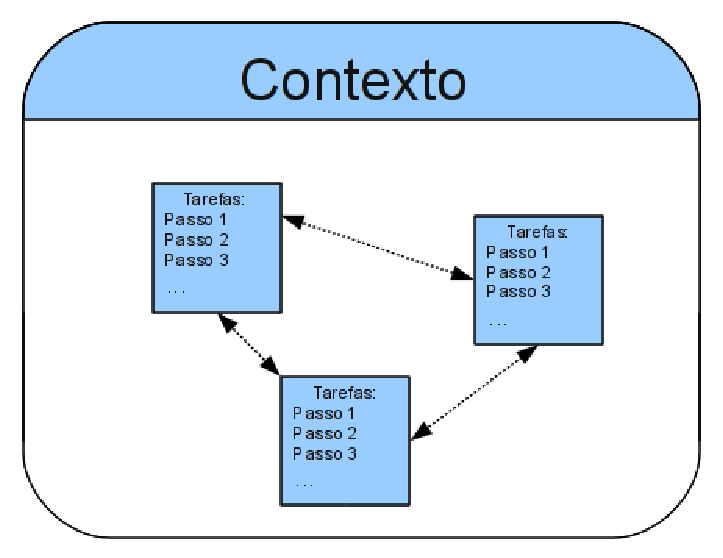
\includegraphics[scale=0.8]{imagens/contexto_agente.eps}}
  \caption{Agentes em um determinado contexto.}
\label{fig:contexto_agente}
\end{figure}

	O contexto aqui chamado é uma plataforma onde o agende executa. Um agente por si só não possui a propriedade de execução, para isto ele necessita de um ambiente propício, onde seu ciclo de vida possa ser controlado (criação e exclusão do agente) e este execute suas tarefas. Uma outra maneira de se enxergar o contexto de execução do agente seria a de um \textit{framework} onde os agentes poderiam ser instalados e executados. Sendo assim, um agente existe apenas naquele determinado contexto no qual ele foi criado, seu ciclo de vida (criação, execução e exclusão) se restringe sempre à plataforma de execução.
	
	Um tipo em especial de agente são os Agentes Móveis. Para essa tipo de agente, uma característica importante a destacar é que ele pode-se mover para um contexto diferente do qual foi originalmente criado. Isso significa que o agente deixou de ter como limitação aquela plataforma à qual ele existia num momento inicial e ganhou a possibilidade de se mover para outros contextos, caso isso seja necessário durante o seu ciclo de vida. 
	
	Algumas utilidades que ajudam a ilustrar os benefícios de se migrar um agente para um contexto diferente do original podem ser citadas a seguir:
	\begin{itemize}
		\item Aproximação do processo com a sua base de dados, diminuindo o tráfego de dados pela rede;
		\item Mudança da máquina a ser utilizada pelo processo, seja por motivos de manutenção ou para se aproveitar de um \textit{hardware} mais poderoso ou mesmo um periférico específico;
		\item Distribuição do processo entre vários \textit{hosts}, etc.
	\end{itemize}

	Conforme ilustrado na Figura~\ref{fig:migrando_agente}, um agente que existia previamente em um contexto A pode, a qualquer momento de sua vida, migrar para um outro contexto B. Para isto basta que exista um meio de ligação entre os dois \textit{hosts} (uma rede de computadores) e a existência do contexto anfitrião propício a receber o agente móvel.

\begin{figure}[htb]
  \centering
  \centerline{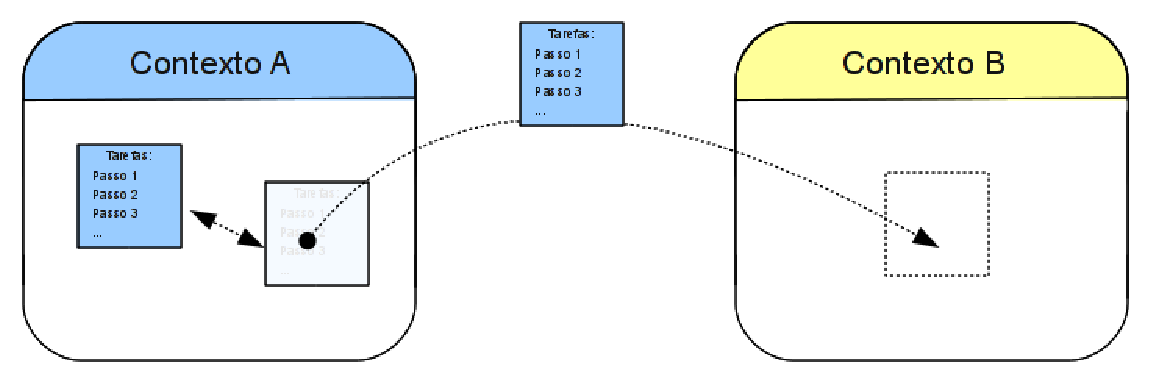
\includegraphics[scale=0.8]{imagens/migrando_agente.eps}}
  \caption{Agente migrando para um contexto diferente do original.}
\label{fig:migrando_agente}
\end{figure}

\section{Mobilidade Forte e Mobilidade Fraca}
	
	Durante uma migração um agente móvel leva consigo todos os dados referentes à execução, além do seu código executável. Em sua concepção original, um agente móvel, ao migrar, deve interromper sua execução no ponto onde ela estiver, encapsular todos os dados referentes ao processo, migrar para o seu destino e, ao chegar, continuar o processamento do ponto onde ele parou. A este modelo de migração, onde o processamento do agente continua no exato ponto onde parou antes da migração, dá-se o nome de Mobilidade Forte.

	Um segundo tipo de migração é a Mobilidade Fraca. Na mobilidade fraca, ao se migrar para um novo contexto, o agente encapsula todas as variáveis globais do processo, porém não continua o processo do exato ponto onde parou, mas sim recomeça o processamento desde o início.

	Para melhor ilustrar esse comportamento. Considere, no seguinte exemplo, que para o dado código, exatamente após a terceira interação, o agente mova do contexto A para o contexto B:
\begin{table}
\lstset{language=C}
\begin{lstlisting}
		for(int i = 0 ; i < 5 ; i++) {
			printf("%i,",i);
		}
\end{lstlisting}
	
\end{table}


	Sendo assim, existirá dois comportamentos distintos para migrações baseadas em Mobilidade Forte e mobilidade Fraca, conforme a tabela~\ref{tabela_mobilidade}.
\begin{table}
\begin{center}
	\begin{tabular}{| c | c | c |}
		\hline
		Tipo & Contexto A & Contexto B \\ \hline
		Mobilidade Fraca & 0, 1, 2, & 0, 1, 2, 3, 4, \\ \hline
		Mobilidade Forte & 0, 1, 2, & 3, 4, \\ \hline
	\end{tabular}
	\caption{Saída de terminal para o código citado em diferentes tipos de migração.}
	\label{tabela_mobilidade}
\end{center}
\end{table}

	Como pode ser notado com base nas saídas de terminal para ambos os tipos de mobilidade, na Mobilidade Fraca a iteração é interrompido antes da migração, mas recomeça a partir do zero ao chegar no seu novo contexto. Já no caso da Mobilidade Forte a iteração, após ser interrompida retoma o seu processamento no novo contexto a partir do exato ponto onde este foi interrompido no contexto original. A biblioteca de agentes móveis \textit{Aglets}, utilizada para esse trabalho, suporta apenas Mobilidade Fraca. Mais detalhes sobre esse assunto serão discutidos posteriormente, na seção sobre \textit{Aglets}.


\section{Agentes Móveis em Java e a Biblioteca \textit{Aglets}}

	Por possuir um código que é executado sobre uma máquina virtual, o Java naturalmente provêem uma camada de abstração para o código a ser executado. Isso significa que, tendo o interpretador Java devidamente instalando em computadores com diferentes sistemas operacionais ou até mesmo baseados em diferentes arquiteturas, têm-se a garantia de que o código será executado da mesma forma, independente do hardware ou ou da plataforma em cada um dos \textit{hosts}. Essa característica facilita a criação de agentes móveis, uma vez que, tendo um processo em execução, caso seja necessário transferi-lo para um segundo contexto, não existe a preocupação de traduzir o código. Para isto, basta simplesmente encapsular as variáveis presentes na máquina virtual Java, além do código Java executável, e transferí-los para a máquina destino.
	
	Para abstrair todo o processo de encapsulamento dos dados de um agente e demais processos envolvidos no controle de seu ciclo de vida e mobilidade, é empregado a utilização de bibliotecas que já provêem todas essas funcionalidades para se trabalhar com agentes móveis em Java. Uma dessas bibliotecas, a utilizada neste trabalho, é a \textit{Aglets} (\textit{Agent Applet}). \textit{Aglets} é uma biblioteca desenvolvida pela IBM Tokio \textit{Research Laboratory}, que possibilita a criação de agentes móveis em Java. Um \textit{aglet} é um agente Java capaz de executar suas tarefas e migrar de um \textit{host} para outro, além de prover ferramentas para multiplicação (clonagem), comunicação entre \textit{aglets} e gerenciamento do ciclo de vida (criação e exclusão de um \textit{aglet}). 
	
	Um \textit{aglet} possui o seu ciclo de vida restrito à plataforma de \textit{aglets} provida para o seu funcionamento. Como padrão, a biblioteca \textit{Aglets} utiliza o servidor \textit{Tahiti} como plataforma de execução dos agentes \textit{aglets} (Figura~\ref{fig:tahiti})\cite{ManualAglets}.

\begin{figure}[htb]
  \centerline{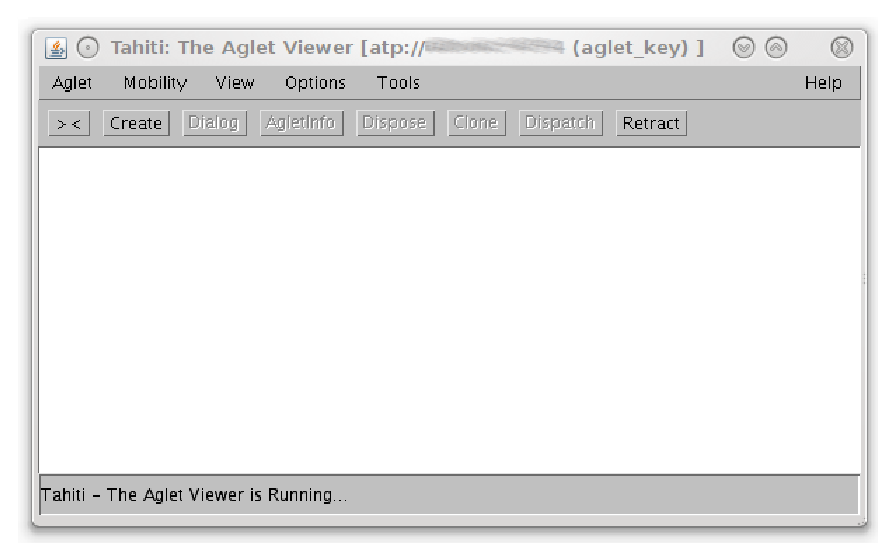
\includegraphics[scale=0.6]{imagens/tahiti.eps}}
  \caption{Servidor de \textit{Aglets Tahiti}.}
\label{fig:tahiti}
\end{figure}

	O \textit{Tahiti} provê a interface para se trabalhar com \textit{aglets}. Através do servidor \textit{Tahiti} pode-se criar e manipular os agentes. Existe também a possibilidade de se utilizar o \textit{Tahiti} sem a interface gráfica através do console(Figura~\ref{fig:tahiti_nogui}).

\begin{figure}
  \centerline{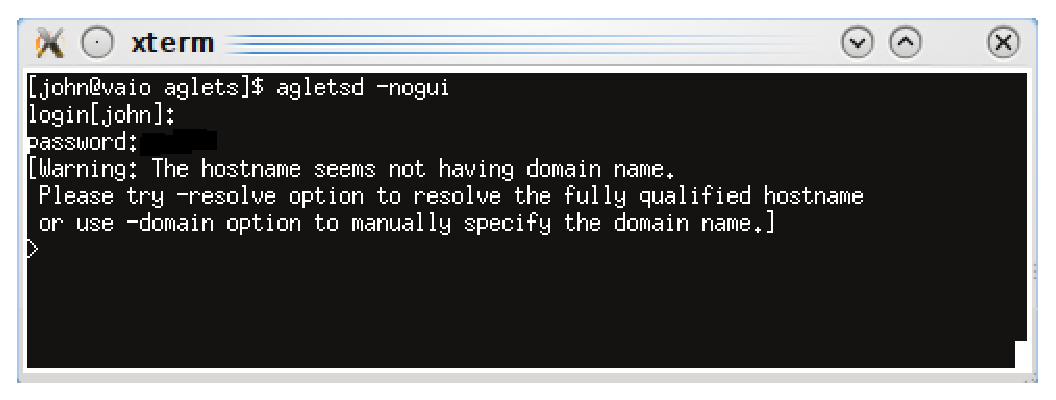
\includegraphics[scale=0.6]{imagens/tahiti-nogui.eps}}
  \caption{Servidor \textit{Tahiti} por linha de comandos.}
\label{fig:tahiti_nogui}
\end{figure}

	Todo agente \textit{aglet} é um objeto derivado da classe pai abstrata \textit{Aglet}. Ao se criar um \textit{aglet}, os métodos pré-definidos são sobrescritos com o código conveniente, a fim de se criar a aplicação desejada. Uma vez desenvolvidos os agentes \textit{aglets}, utiliza-se o servidor \textit{Tahiti} para iniciar o ciclo de vida dos agentes.


\section{Ciclo de Vida \textit{Aglets}}

	Todo agente possui um ciclo de vida definido dentro de seu contexto. Conforme ilustrado na Figura~\ref{fig:ciclo}, um \textit{aglet} possui cinco principais fases durante o seu ciclo de vida:
\begin{itemize}

	\item Criação: Ocorre uma única vez em todo o ciclo de vida do \textit{aglet}. Ao ser criado, um \textit{aglet} invoca o método \textit{onCreation}() e executa o conteúdo deste método. O método \textit{onCreation}() é um método abstrato da classe pai \textit{Aglet} e deve ser sobrescrito pelo agente.

	\item Execução: A execução (método \textit{run}()) de um \textit{aglet} acontece em três momentos distintos em seu ciclo de vida: após sua criação (logo após a execução do método \textit{onCreation}()), após uma migração (assim que o agente chega ao \textit{host}) e após uma clonagem, executado apenas pelo novo agente (o original continua o seu ciclo de execução natural). A execução é invocada através do método \textit{run}(), também herdado da classe pai \textit{Aglet} e que também deve ser sobrescrito.

	\item Clonagem:  Após uma clonagem, o agente original cria uma cópia idêntica de si. Esta cópia executa os métodos referentes ao clone \textit{listener} do agente e em seguida executa o método \textit{run}() referente. Após criado, o clone segue um ciclo de vida completamente independente do agente original.

	\item Migração: Um método que se move de um contexto para outro carrega consigo todas as informação do momento anterior à migração. Ao chegar em seu novo \textit{host}, o agente que executou a migração trata os eventos referentes ao \textit{Mobility Listener} e em seguida executa o método \textit{run}(). Como o método \textit{run}() é executado a partir de seu início, toda a execução que porventura estava sendo executada dentro deste método antes da migração será refeita. Por esse motivo é que a migração de um agente \textit{Aglet} é considerada do tipo Mobilidade Fraca.

	\item Exclusão: O final da vida de um \textit{aglet} não se dá ao final da execução do método \textit{run}(), mas sim deve ser explicitamente chamado. Caso contrário, o agente permanece no seu referente contexto.
\end{itemize}
\begin{figure}[htb]
  \centering
  \centerline{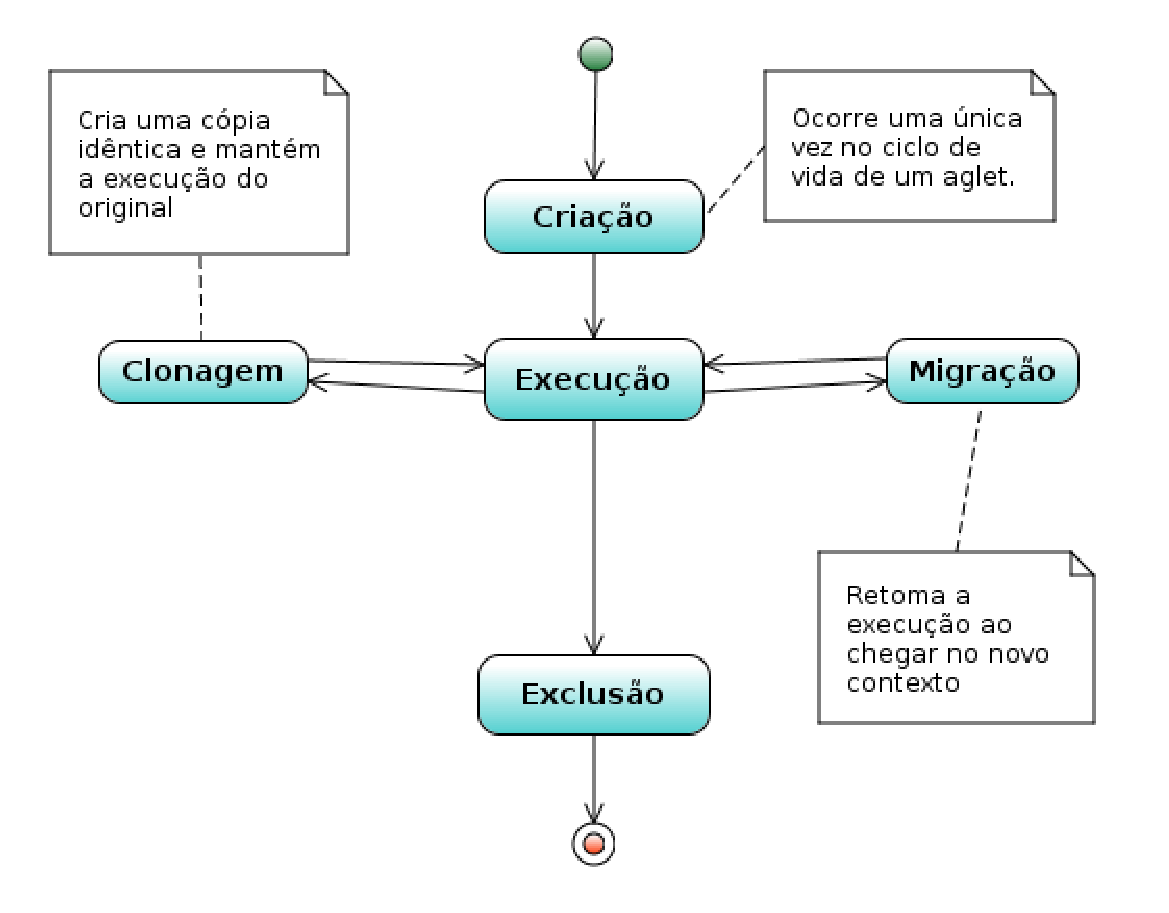
\includegraphics[scale=0.6]{imagens/ciclo_vida_aglet.eps}}
  \caption{Ciclo de vida de um \textit{aglet}.}
\label{fig:ciclo}
\end{figure}	


\section{Comunicação Entre \textit{Aglets}}

	Agentes comunicam entre si através de mensagens. Essas mensagens são enviadas de um agente para outro através de \textit{proxys}. Um \textit{proxy} pode ser visto neste caso como uma interface de comunicação entre agentes, que proporciona transparência e segurança na comunicação entre os \textit{aglets}. Para que um \textit{aglet} se comunique com outro, basta ter o seu \textit{proxy} remoto, mascarando assim a real localização do agente.
	
	Todo agente possui um identificador único e é através desse identificador e da URL onde o agente se encontra que se obtém o \textit{proxy} possibilitando a comunicação.
	
	O método \texttt{handleMessage(Message msg)} é responsável por tratar as mensagens recebidas pelos agentes. Esse método recebe como parâmetro um objeto do tipo \textit{Message} que contém os dados da mensagem. O objeto Message possui dois principais atributos como ilustra o diagrama da Figura~\ref{fig:classe_message}. O atributo \textit{kind} é uma \textit{string} e contém o tipo da mensagem, um rótulo. O atributo \textit{arg} é um objeto que pode ser enviado através da mensagem. Este objeto deve ser serializável para que possa ser enviado através de uma mensagem.


	Ao receber uma mensagem, o método \textit{handleMessage}(...) trata a mensagem com base em seu rótulo (\textit{kind}). Toda a comunicação entre os agentes, mesmo os que estão no mesmo contexto, é feita através de mensagens e, consecutivamente, através dos \textit{proxys} dos \textit{aglets}. Veja a Figura~\ref{fig:classe_message}

\begin{figure}[htb]
  \centering
  \centerline{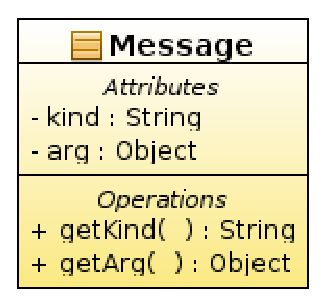
\includegraphics[scale=0.7]{imagens/classe_message.eps}}
  \caption{Classe Message.}
\label{fig:classe_message}
\end{figure}

 

\section{Considerações Finais}

	As propriedades de mobilidade e independência dos agentes móveis proporcionam características que podem ser exploradas na implementação de aplicações distribuídas. O fato de um agente poder se mover por diferentes \textit{hosts} em tempo de execução, por exemplo, pode ser usado como forma de balanceamento de cargas, ou simplesmente para manter processos que trocam muitas mensagens fisicamente perto, em uma mesma rede, agilizando assim o tráfego de dados na rede. A facilidade proporcionada para a troca de mensagens e envio de objetos encapsulados dentro dessas mensagens também pode ser utilizada para enviar eventos de um nó de uma rede de processamento para outro, ou enviar eventos que foram gerados em um processo para serem tratados por outro processo. 
	
	É com base nessas e em outras características de agentes móveis e da biblioteca \textit{Aglets} que a implementação do protocolo \textit{Rollback} Solidário deste trabalho foi desenvolvida, a fim de se avaliar a viabilidade da implementação de um software de simulação distribuída utilizando das propriedades dos agentes móveis e, mais especificamente neste caso, da linguagem Java e da biblioteca \textit{Aglets}.



